%%%%%%%%%%%%%%%%% document setup %%%%%%%%%%%%%%%%%

% Don't like 10pt? Try 11pt or 12pt
\documentclass[10pt]{article}

% The automated optical recognition software used to digitize resume
% information works best with fonts that do not have serifs. This
% command uses a sans serif font throughout. Uncomment both lines (or at
% least the second) to restore a Roman font (i.e., a font with serifs).
%\usepackage{times}
%\renewcommand{\familydefault}{\sfdefault}

% This is a helpful package that puts math inside length specifications
\usepackage{calc}
\usepackage{comment}
\usepackage{graphicx}
\graphicspath{ {.} }

% Simpler bibsection for CV sections
% (thanks to natbib for inspiration)
\makeatletter
\newlength{\bibhang}
\setlength{\bibhang}{1em} %1em}
\newlength{\bibsep}
{\@listi \global\bibsep\itemsep \global\advance\bibsep by\parsep}
\newenvironment{bibsection}%
{\begin{enumerate}{}{%
			%        {\begin{list}{}{%
			\setlength{\leftmargin}{\bibhang}%
			\setlength{\itemindent}{-\leftmargin}%
			\setlength{\itemsep}{\bibsep}%
			\setlength{\parsep}{\z@}%
			\setlength{\partopsep}{0pt}%
			\setlength{\topsep}{0pt}}}
	{\end{enumerate}\vspace{-.6\baselineskip}}
%        {\end{list}\vspace{-.6\baselineskip}}
\makeatother

% Layout: Puts the section titles on left side of page
\reversemarginpar

%
%         PAPER SIZE, PAGE NUMBER, AND DOCUMENT LAYOUT NOTES:
%
% The next \usepackage line changes the layout for CV style section
% headings as marginal notes. It also sets up the paper size as either
% letter or A4. By default, letter was used. If A4 paper is desired,
% comment out the letterpaper lines and uncomment the a4paper lines.
%
% As you can see, the margin widths and section title widths can be
% easily adjusted.
%
% ALSO: Notice that the includefoot option can be commented OUT in order
% to put the PAGE NUMBER *IN* the bottom margin. This will make the
% effective text area larger.
%
% IF YOU WISH TO REMOVE THE ``of LASTPAGE'' next to each page number,
% see the note about the +LP and -LP lines below. Comment out the +LP
% and uncomment the -LP.
%
% IF YOU WISH TO REMOVE PAGE NUMBERS, be sure that the includefoot line
% is uncommented and ALSO uncomment the \pagestyle{empty} a few lines
% below.
%

%% Use these lines for letter-sized paper
\usepackage[paper=letterpaper,
%includefoot, % Uncomment to put page number above margin
marginparwidth=1.2in,     % Length of section titles
marginparsep=.05in,       % Space between titles and text
margin=1in,               % 1 inch margins
includemp]{geometry}

%% Use these lines for A4-sized paper
%\usepackage[paper=a4paper,
%            %includefoot, % Uncomment to put page number above margin
%            marginparwidth=30.5mm,    % Length of section titles
%            marginparsep=1.5mm,       % Space between titles and text
%            margin=25mm,              % 25mm margins
%            includemp]{geometry}

%% More layout: Get rid of indenting throughout entire document
\setlength{\parindent}{0in}

\usepackage[shortlabels]{enumitem}

%% Reference the last page in the page number
%
% NOTE: comment the +LP line and uncomment the -LP line to have page
%       numbers without the ``of ##'' last page reference)
%
% NOTE: uncomment the \pagestyle{empty} line to get rid of all page
%       numbers (make sure includefoot is commented out above)
%
\usepackage{multicol}
\usepackage{fancyhdr,lastpage}
\pagestyle{fancy}
%\pagestyle{empty}      % Uncomment this to get rid of page numbers
\fancyhf{}\renewcommand{\headrulewidth}{0pt}
\fancyfootoffset{\marginparsep+\marginparwidth}
\newlength{\footpageshift}
\setlength{\footpageshift}
{0.5\textwidth+0.5\marginparsep+0.5\marginparwidth-2in}
\lfoot{\hspace{\footpageshift}%
	\parbox{4in}{\, \hfill %
		\arabic{page} of \protect\pageref*{LastPage} % +LP
		%                    \arabic{page}                               % -LP
		\hfill \,}}

% Finally, give us PDF bookmarks
\usepackage{color,hyperref}
\definecolor{darkblue}{rgb}{0.0,0.0,0.3}
\hypersetup{colorlinks,breaklinks,
	linkcolor=darkblue,urlcolor=darkblue,
	anchorcolor=darkblue,citecolor=darkblue}

%%%%%%%%%%%%%%%%%%%%%%%% End Document Setup %%%%%%%%%%%%%%%%%%%%%%%%%%%%


%%%%%%%%%%%%%%%%%%%%%%%%%%% Helper Commands %%%%%%%%%%%%%%%%%%%%%%%%%%%%

% The title (name) with a horizontal rule under it
% (optional argument typesets an object right-justified across from name
%  as well)
%
% Usage: \makeheading{name}
%        OR
%        \makeheading[right_object]{name}
%
% Place at top of document. It should be the first thing.
% If ``right_object'' is provided in the square-braced optional
% argument, it will be right justified on the same line as ``name'' at
% the top of the CV. For example:
%
%       \makeheading[\emph{Curriculum vitae}]{Your Name}
%
% will put an emphasized ``Curriculum vitae'' at the top of the document
% as a title. Likewise, a picture could be included:
%
%   \makeheading[\includegraphics[height=1.5in]{my_picutre}]{Your Name}
%
% the picture will be flush right across from the name.
\newcommand{\makeheading}[2][]%
{\hspace*{-\marginparsep minus \marginparwidth}%
	\begin{minipage}[t]{\textwidth+\marginparwidth+\marginparsep}%
		{\large \bfseries #2 \hfill #1}\\[-0.15\baselineskip]%
		\rule{\columnwidth}{1pt}%
	\end{minipage}}
	
	% The section headings
	%
	% Usage: \section{section name}
	\renewcommand{\section}[1]{\pagebreak[3]%
		\hyphenpenalty=10000%
		\vspace{1.3\baselineskip}%
		\phantomsection\addcontentsline{toc}{section}{#1}%
		\noindent\llap{\scshape\smash{\parbox[t]{\marginparwidth}{\raggedright #1}}}%
		\vspace{-\baselineskip}\par}
	
	% An itemize-style list with lots of space between items
	\newenvironment{outerlist}[1][\enskip\textbullet]%
	{\begin{itemize}[#1,leftmargin=*]}{\end{itemize}%
		\vspace{-.6\baselineskip}}
	
	% An environment IDENTICAL to outerlist that has better pre-list spacing
	% when used as the first thing in a \section
	\newenvironment{lonelist}[1][\enskip\textbullet]%
	{\begin{list}{#1}{%
				\setlength{\partopsep}{0pt}%
				\setlength{\topsep}{0pt}}}
		{\end{list}\vspace{-.6\baselineskip}}
	
	% An itemize-style list with little space between items
	\newenvironment{innerlist}[1][\enskip\textbullet]%
	{\begin{itemize}[#1,leftmargin=*,parsep=0pt,itemsep=0pt,topsep=0pt,partopsep=0pt]}
		{\end{itemize}}
	
	% An environment IDENTICAL to innerlist that has better pre-list spacing
	% when used as the first thing in a \section
	\newenvironment{loneinnerlist}[1][\enskip\textbullet]%
	{\begin{itemize}[#1,leftmargin=*,parsep=0pt,itemsep=0pt,topsep=0pt,partopsep=0pt]}
		{\end{itemize}\vspace{-.6\baselineskip}}
	
	% To add some paragraph space between lines.
	% This also tells LaTeX to preferably break a page on one of these gaps
	% if there is a needed pagebreak nearby.
	\newcommand{\blankline}{\quad\pagebreak[3]}
	\newcommand{\halfblankline}{\quad\vspace{-0.5\baselineskip}\pagebreak[3]}
	
	% Uses hyperref to link DOI
	\newcommand\doilink[1]{\href{http://dx.doi.org/#1}{#1}}
	\newcommand\doi[1]{doi:\doilink{#1}}
	
	% For \url{SOME_URL}, links SOME_URL to the url SOME_URL
	\providecommand*\url[1]{\href{#1}{#1}}
	% Same as above, but pretty-prints SOME_URL in teletype fixed-width font
	\renewcommand*\url[1]{\href{#1}{\texttt{#1}}}
	
	% For \email{ADDRESS}, links ADDRESS to the url mailto:ADDRESS
	\providecommand*\email[1]{\href{mailto:#1}{#1}}
	% Same as above, but pretty-prints ADDRESS in teletype fixed-width font
	%\renewcommand*\email[1]{\href{mailto:#1}{\texttt{#1}}}
	
	%\providecommand\BibTeX{{\rm B\kern-.05em{\sc i\kern-.025em b}\kern-.08em
	%    T\kern-.1667em\lower.7ex\hbox{E}\kern-.125emX}}
	%\providecommand\BibTeX{{\rm B\kern-.05em{\sc i\kern-.025em b}\kern-.08em
	%    \TeX}}
	\providecommand\BibTeX{{B\kern-.05em{\sc i\kern-.025em b}\kern-.08em
			\TeX}}
	\providecommand\Matlab{\textsc{Matlab}}
%%%%%%%%%%%%%%% end docuemnt setup %%%%%%%%%%%%%%%






%%%%%%%%%%%%%%% begin my cv document %%%%%%%%%%%%%%%

\begin{document}
\makeheading %[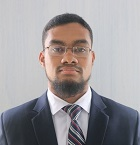
\includegraphics{mahmud1}]
{Abdullah Al Mahmud}

\section{Contact Information}
\newlength{\rcollength}\setlength{\rcollength}{1.4in}%

\begin{tabular}[t]{@{}p{\textwidth-\rcollength}p{\rcollength}}
	Flat: B-19, Kortoa Building, Pabna Cadet College   & +880-1722-437040 \\
	Pabna, Bangladesh     & \email{almahmud.sbi@gmail.com}\\
	& \href{https://mahmud.bishwo.com/}{Website} \href{https://github.com/mahmudstat}{Github} 
\end{tabular}


\section{Research Interest}
Probability, Statistical Inferfence, and Machine Learning


\section{Education}
\begin{outerlist}
	\item[] MS in Statistics
		\begin{innerlist}
			\item University of Dhaka (2018-2019)
			\item CGPA: 2.71 (out of 4)
		\end{innerlist}
	
	\item[] B.S. in Statistics
		\begin{innerlist}
			\item University of Dhaka (2012-2017)
			\item Project: \emph{An Insight into Induced Seismicity in Bangladesh.}
			\item Advisor: {Md. Ahsan Uddin}
			\item CGPA: 3.31 (out of 4)
		\end{innerlist}
		
	\item[] Higher Secondary School Certificate
	\begin{innerlist}
		\item Dhaka Board (July 2010)
		\item Udayan Higher Secondary School
		\item GPA: 5.00 (out of 5)
	\end{innerlist}
	
	\item[] Secondary School Certificate
		\begin{innerlist}
			\item Cumilla Board (May 2008)
			\item Poura Shahid Smrity Academy
			\item GPA: 5.00 (out of 5)
		\end{innerlist}

	\item[] \textbf{Test Scores}
		\begin{innerlist}
			\item \textbf{GRE:} 309 (Quantitative: 160, Verbal: 149)
			\item \textbf{TOEFL:} 89 (Reading: 24, Listening: 21, Speaking: 21 , Wriitng: 23 )
		\end{innerlist}
\end{outerlist}



\section{Major Courses}

%%multi start
    \begin{multicols}{3}
    \begin{itemize}
	\item Introduction to Statistics
	\item Probability
	\item Linear Algebra
	\item Calculus
	\item Mathematical Analysis
	\item Simulations
	\item Theory of Estimation
	\item  Regression Analysis
	\item Operations Research
	\item Multivariate Analysis
	\item Stochastic Process
	\item Time Series Analysis
	\item Biostatistics
	\item Robust Statistics
	\item Artificial Intelligence
	\item Design and Analysis of Experiment
    \end{itemize}
    \end{multicols}
%%multi 


\section{Professional Experience}
\flushleft
\textbf{Lecturer (statistics)} \hfill{October 2019 - Present}
	\begin{innerlist}
		\item[]{Engineears and Advisors Ltd. (EAL)/ Dhaka/ Bangladesh}
	\end{innerlist}
\textbf{Research Asistantr} \hfill{September 2019 - October 2019}
	\begin{innerlist}
		\item[]{Engineears and Advisors Ltd. (EAL)/ Dhaka/ Bangladesh}
	\end{innerlist}
\textbf{Science Contributor} \hfill{October 2016 -  August 2019}
	\begin{innerlist}
		\item[]{\href{https://www.prothomalo.com/}{The Daily Prothom Alo}/ Dhaka/ Bangladesh}
	\end{innerlist}
\textbf{Content Developer} \hfill{November 2017 - August 2019}
	\begin{innerlist}
		\item[]{\href{https://srcbd.org/srcbd_team}{Statistical Research Consultants, Bangladesh}/ Dhaka/ Bangladesh}
	\end{innerlist}




%\section{Submitted Journal Publications}
%\begin{bibsection}
%	\vspace{-.1275in}
%	\item {\bf Hasan, M.}, Asiful, H., "Recognizing and tracking people by their gait signatures across multiple non-intersecting surveillance cameras." \emph{IEEE}, 52(8):25--31, 2018.t...
%\end{bibsection}

%\section{Peer-Reviewed Conference Paper}
%\vspace{-.1in}
%\begin{bibsection}
%	\item {\bf Hasan, M.}, Asiful, H. "preparing journal paper or published conference paper"
%\end{bibsection}




%\section{Achievements}
%{\bf B.Sc. Engineering Scholarships}
%\begin{innerlist}
%	\item[] KUET students merit scholarships through four years for academic
%	excellence from the Govt. of the People's Republic of Bangladesh
%\end{innerlist}


\section{Conference Papers}
\begin{innerlist}
	\item Mahmud, A, A and Rahman, M, M. Goodness of fit for uniform distribution: Benford's law method. National Conference on Applications of Statistics on Sustainable Development Goals, MBSTU-2018, 24 September 2018. ID: TS3-11, Tangail, Bangladesh.
\end{innerlist}

\section{Accepted Papers}
\begin{innerlist}
	\item Mahmud, A, A . 2018. {Testing of Compliance of Benford’s Law with Disaster Death Tolls.} 
\\Journal of Bangladesh Cadet College. 
\end{innerlist}


\section{Other Researches \newline
(Unpublished)}
\begin{innerlist}
	\item An Insight into the Concept and Applictaions of Negative Probability.
	\item Prediction of Rainfall Pattern in Bangladesh Using Machine Learning Algorithms. 
	\item An Insight into Induced Seismicity in Bangladesh.
\end{innerlist}

\section{Professional Research}
\textbf{Feasibility Study} \hfill{November, 2018}
	\begin{innerlist}
		\item[]{Dhaka-Chattogram High-speed Rail Project}
	\end{innerlist}
\textbf{Social Media Trend Analysis of Youth Students} \hfill{January, 2019}
	\begin{innerlist}
		\item[]{Project by Move Foundation}
	\end{innerlist}



\section{Technical Skills}
\begin{innerlist}
	\item[] Programming Languages: \hfill {FORTRAN, Bash} \\
	\item[] Statistical  Programming: \hfill {R} \\
	\item[] Statistical Packages: \hfill {STATA, SPSS, TABLEAU} \\
	\item[] Database: \hfill {SQL} \\
	\item[] Geospatial Framework: \hfill {GIS (with R)} \\
	\item[] Dopcument Processing: \hfill {MS Office, Libreoffice, Markdown, Latex} \\
	\item[] Internet Skills: \hfill {MathJax, HTML, CSS, SVG, JS} \\
\end{innerlist}

%Workshop, training, course, leadership certificate, scholarship etc...

\section{Books}
\textbf{Benglai Translation of \href{https://www.facebook.com/brieferhist} {\textit A Briefer History of Time} \hfill{2017 Ekushey Book Fair}}
	\begin{innerlist}
		\item[]{ Authored by Stephen Hawking and Leonard Mlodino}
	\end{innerlist}
\flushleft
 \href{https://ms.bishwo.com/}{\textbf{Mohabishwer Simana (Edge of the Universe)}} \hfill{2019 Ekushey Book Fair}

\flushleft
\href{https://os.bishwo.com/} { \textbf{Osim Somikoron (The Infinite Equation)}} \hfill{2019 Ekushey Book Fair}


\section{Workshops}
\begin{innerlist}
	\item {\textbf {July 2018:} Day long workshop on \textit{Statistics for Research} by Dr. Rahmatull Imon, professor, Ball State University, USA. } 
	\item {\textbf{December 2014:} Abdul Jabbar Workshop on Astronomy and Cosmology.} 
	\item {\textbf{June 2016:} Astronomy Workshop conducted by BAA and Russian Cultural Centre, Dhaka.} 
\end{innerlist}

\section{Online Courses}
\textbf{Coursera} \hfill{August 2020}
	\begin{innerlist}
		\item[]\href{https://www.coursera.org/learn/introduction-git-github/home/welcome} {Introduction to Git and GitHub
}
	\end{innerlist}
\textbf{Courserap} \hfill{May 2020}
	\begin{innerlist}
		\item[]\href{https://www.coursera.org/learn/linux-tools-for-developers/home/welcome} {Linux Tools for Developers
}
	\end{innerlist}
\textbf{Data Camp} \hfill{June 2018}
	\begin{innerlist}
		\item[]\href{https://www.datacamp.com/courses/supervised-learning-in-r-classification} {Supervised Learning in R: Classification}
	\end{innerlist}
%
%\flushleft
%\textbf{Data Camp} \hfill{October 2018}
%	\begin{innerlist}
%		\item[]\href{https://www.datacamp.com/courses/generalized-linear-models-in-r} {Generalized Linear Models in R}
%	\end{innerlist}

%\flushleft
%\textbf{Coursera} (Johns Hopkins University) \hfill{January 2018}
%	\begin{innerlist}
%		\item[]\href{https://www.coursera.org/account/accomplishments/records/WPS6M6WNTSBT} {The Data %Scientist\textsc{\char13}s Toolbox} 
%	\end{innerlist}

%\flushleft
%\textbf{Coursera} (University of California, Irvine) \hfill{February 2018}
%	\begin{innerlist}
%		\item[]\href{https://www.coursera.org/account/accomplishments/records/PK7RR7KUB9K} {Grammar and Punctuation}
%	\end{innerlist}

%\flushleft
%\textbf{Coursera} (Johns Hopkins University) \hfill{February 2018}
%	\begin{innerlist}
%		\item[]\href{https://www.coursera.org/account/accomplishments/records/BK4MG2X9WJT} {A Crash Course in Data Science}
%	\end{innerlist}

%\flushleft
%\textbf{Coursera} (University of California, DAVIS) \hfill{October 2018}
%	\begin{innerlist}
%		\item[]{Fundamentals of GIS}
%	\end{innerlist}

%\flushleft
%\textbf{Coursera} (Georgia Institute of Technology) \hfill{February 2018}
%	\begin{innerlist}
%		\item[]\href{https://www.coursera.org/account/accomplishments/records/C97LRRJGMWXL} {Write Professional Emails in English}
%	\end{innerlist}


\section{Kaggle Competitions}
	\begin{innerlist}
	\item[] \textbf{Titanic: Machine Learning from Disaster} \hfill{Accuracy: 76.55\%}
	\item[] \textbf{Digit Recognizer} \hfill{Accuracy: 53\%}
	\item[] \textbf{Gouse Price Prediction} \hfill{Accuracy: 92\%}
	\end{innerlist}

\section{Extra-Curricular Activities}
\begin{innerlist}
	\item Member at Dhaka University Science Society (DUSS), University of Dhaka.
	\item Writer at National Science Magazines, including BigganChinta.
	\item Regular Public lectures on Mathematics and Astronomy
	\item Writing for \href {https://www.en.wikipedia.org}{Wikipedia}
\end{innerlist}

\section{Leadership skills}
\begin{innerlist}
	\item {Led a team of 11 members in a research project in fourth year } 
	\item {Was a coordinator of \href{http://scholarsforumdhaka.org/} {Scholar\textsc{\char13}s Forum}, a student welfare organization.}
	\item {Coordinated Science Writers\textsc{\char13} cell, a platform of Bengali Science Writers.} 
\end{innerlist}

\section{Language Skills}
\begin{innerlist}
	\item[] Bengali: \hfill {Mother Tongue} \\
	\item[] English: \hfill {Fluent in all areas} \\
	\item[] Arabic: \hfill {Introductory} \\
\end{innerlist}

\section{References}

{\bf Dr. Md. Jafar Ahmed Khan}
\begin{innerlist}
	\item[] \href{http://www.du.ac.bd/faculty/faculty_details/STA/216} {Professor, Department of Statistics} \\
	\href{http://www.du.ac.bd/} {University of Dhaka}\\
	Dhaka - 1000, Bangladesh \\
    E-mail: jafar@du.ac.bd  \hfill {Phone: 880-2-9661900/7219, +8801965350939}
\end{innerlist}

\halfblankline

{\bf Dr. Wasimul Bari}
\begin{innerlist}
	\item[]  \href{http://www.du.ac.bd/faculty/faculty_details/STA/217} {Professor, Department of Statistics} \\
	\href{http://www.du.ac.bd/} {University of Dhaka}\\
	Dhaka - 1000, Bangladesh \\
    E-mail: w\_bari@du.ac.bd  \hfill {Phone: 880-2-9661900/7191, +8801747424348}
\end{innerlist}

\halfblankline

{\bf Dr. Taslim Sazzad Mallick}
\begin{innerlist}
	\item[] Associate Professor, {Department of Statistics} \\
	\href{http://www.du.ac.bd/} {University of Dhaka}\\
	Dhaka - 1000, Bangladesh \\
    E-mail: tsmallick@du.ac.bd  \hfill {Phone: 880-2-9661900, 9001321, +8801747424348}
\end{innerlist}

\end{document}












